\documentclass[a4paper]{article}
%%%%%%%%%%%%%%%%%%% TODO: change k to \mathbf{k}

\usepackage[utf8]{inputenc}
\usepackage[T1]{fontenc}
\usepackage{textcomp}
\usepackage[english]{babel}
\usepackage{amsmath, amssymb, amsfonts}
\usepackage{physics}


% figure support
\usepackage{import}
\usepackage{xifthen}
\pdfminorversion=7
\usepackage{pdfpages}
\usepackage{transparent}
\newcommand{\hcut}{\hbar}
\newcommand{\incfig}[1]{%
	\def\svgwidth{\columnwidth}
	\import{./figures/}{#1.pdf_tex}
}
\newcommand{\tensor}[1]{\overset{\leftrightarrow}{#1}}

\pdfsuppresswarningpagegroup=1

\title{Physics of Quantum Devices}
\date{}
\begin{document}
\maketitle
\section*{Kinetic Theory of Gases}
\textbf{Kinetic theory} is concerned with the marcoscopic properties
of large numbers of particles, starting from their classical equations
of motion. This course then goes on to develop the semiclassical, and
quantum pictures.

Phenomenological thermodynamics is fine and all, but there is a way
of creating a much more satisfactory \emph{emergent} theory. The
following need to be outlined
\begin{itemize}
	\item definition of ``equilibrium" for moving particles
	\item whether all systems evolve towards equilibrium
	\item time evolution of non-equilibrium systems
\end{itemize}

Start with something like the ideal gas. $N$-particle system, generalized
coordinates $\left\{ \vec{q}_i(t), \vec{p}_i(t) \right\} \forall i \in N$.
A microstate $\mu(t) \in \Gamma$, where $\Gamma$ is the $6N$-dimensional
phase space, evolves according to
\begin{equation} \label{micro}
	\begin{cases}
		&\frac{\dd \vec{q}_i}{\dd t} = \frac{\dd \mathcal{H}}{\dd \vec{p}_i} \\
		&\frac{\dd \vec{p}_i}{\dd t}= -\frac{\dd \mathcal{H}}{\dd \vec{q}_i}
	\end{cases},
\end{equation}

An important fact to keep in mind is that the microscopic equations
of motion \ref{micro} have \emph{time reversal symmetry}, $\because \mathcal{H}$ is invariant under the transformation $T(\mathbf{p, q}) 
\to (-\mathbf{p, q})$

Representing macrostates requires the introduction of ensembles of
a system.

\section*{Boltzmann Transport Equation}
What exactly does it mean to describe a condensed matter system
outside equilibrium? Reminding us of the Fermi-Dirac distro, in equilibrium
\begin{equation}
	f(\varepsilon) = \frac{1}{1 + \exp((\varepsilon - \mu)\beta)}
\end{equation}

In equilibrium, $\mu(T=0) = \varepsilon_F$, where $\mu$ is the electrochemical potential.
$\varepsilon_F$ reflects the carrier density. If your carrier density
varies, then your electrochemical potential $\mu$ has spatiotemporal
varitaion.

A non-equiilbrium with the distribution still having the same functional
form would have some spatiotemporal variation
\begin{equation}
	f(k,\vec{r},t) = \frac{1}{1 + \exp\left(\left( \varepsilon(k) - \mu(\vec r,t) \right)\beta(\vec{r}, t)\right) }.
\end{equation}

Note that the quantities $T, \mu$ et cetera are defined in equibrium
and do not have any meaning outside of equilibrium. So, the current
problem at hand could use the \emph{local equilibrium approximation}.

In this approximation, we define the equilibrium functions only in
infinitesimal volume elements of the system. Once we are assuming that there are temperature and carrier concentration
gradients, we can at best define particle distribution in a small
volume of the phase space. The form of the function remains the same,
which is basically representative of us taking a local-equilibrium
approximation, and not going too far from equilibrium.

The Fermi energy $\epsilon_F$ is a measure of the carrier density;
$\epsilon_F$ is higher for greater carrier density. Any gradient
in the carrier concentration means that there is going to be a
corresponding gradient in the electrochemical potential.

Now, how would you go about defining current density $\vec{j}$?
Remember Drude model?
\begin{equation}
	\mathbf{j} = nev_d
\end{equation}

Start by calculating the current density being contributed by a small
region of the reciprocal space, estimate the number density occupying
that region using the density of states and then multiply by the
velocity. Integrate over the whole $k$-space to get the total current
density.

A general non-equilibrium system would have spatiotemporally varying
$n$, $v_d$ and all. We can arrive at a current density expression using
the density of states and the distribution function by filling up the
bandstructure/energy levels. We consider the contributiong of electrons
from a small volume element of phase space  $\dd ^3 k$. So, we start
with the product of the spin degeneracy, the density of states in the $k$-space, the carrier charge, the density of states and the velocity. Integrate.
\begin{equation} \label{current_density}
	\begin{split}
		\mathbf{j} &= (-e)2\times \frac{1}{8\pi^3}\int f(k, \mathbf{r}, t)v_n(k)\dd^3k\\
		\implies \mathbf{j} &= -\frac{1}{4\pi^3}\int \dd ^3 k f(k, \mathbf{r}, t)\textbf{v}_n(k)
	\end{split}
\end{equation}

Note that $f = f(k, \mathbf{r}, t)$ is not the equilibrium quantity.
This procedure is fairly general, this we have calculated the charge
current density. Calculation of, say, energy current density would
proceed in a similar manner, i.e. local equilibrium approximation,
contribution from small volume element in the $k$-space and integrate
over the whole $k$-space.

So, we want the `dynamics of the phase space' now that we are out of 
equilibrium.
\begin{equation}
	\label{dfdt}
	\frac{\dd f}{\dd t} = \pdv{f}{t} + \dot{\mathbf{r}}\vdot \grad f + \dot{\textbf{k}}\vdot\grad f
\end{equation}

We know that the expression for velocity in our model is
\begin{equation}
	\label{speed}
	\begin{split}
		\mathbf{v}(\mathbf{k}) &= \frac{1}{\hbar}\grad_k\varepsilon(\mathbf{k})\\
		\text{OR}\quad \dot{\textbf{r}} &= \frac{1}{\hcut}\grad_k\epsilon(\textbf{k}),
	\end{split}
\end{equation}
and the external force is modelled as
\begin{equation}
	\label{force}
	\hbar \dot{\mathbf{k}} = \mathbf{F}
\end{equation}

Substituting equations \ref{force} and \ref{speed} into equation
\ref{dfdt}, we get
\begin{equation}
	\label{dfdt2}
	\frac{\dd f}{\dd t} = \pdv{f}{t} +  \mathbf{v}(\mathbf{k})\vdot\grad_rf + \frac{\mathbf{F}}{\hbar}\vdot\grad_k f
\end{equation}

How does one define steady state? We expect the distribution to remain
static in the steady state, as in
\begin{equation} 
	\label{equil}
	\frac{\dd f}{\dd t} = 0.
\end{equation}

It is easy to see that the first and second terms on the right side
of equation \ref{dfdt2} are zero in steady state. What about the last
one, the force term? Even in equilibrium,  $f = f(\textbf{k})$, and if
we apply some non-zero $\textbf{F}$, we will have a non-zero term.

Think about it this way; if we apply a uniform electric field on an
electron in some band of a nice crystal, will a steady-state be acheived?

The answer is very clearly no, there are no dissipative terms in
equation \ref{dfdt2}. Practical systems have dissipations and all,
scattering off of ions. We could empirically add a collision terms.

To account for collisions we define
\begin{equation}
	\pdv{f}{t} + \vec{v}(\vec{k})\vdot\grad_rf + \frac{\vec{F}}{\hbar}\vdot\grad_k f - \pdv{f}{t}\Bigg|_\text{coll} = \frac{\dd f}{\dd t},
\end{equation}
which at steady state becomes
\begin{equation}
	\label{sstate}
	\pdv{f}{t} + \mathbf{v}_k \vdot \grad_r f + \frac{\textbf{F}}{\hcut}\vdot\grad_k f = \pdv{f}{t}\Bigg|_\text{coll}
\end{equation}

This is the equation that we have to solve for different questions.
Now, recall that we did a problem that showed Bloch oscillations.
We had the Bloch frequency
\begin{equation}
	\omega_B = \left( \frac{eE}{\hbar} a\right) 
\end{equation}
For the parameters $E = 10\text{kV/cm}$,  $a = 1\text{Angstrom}$, we
get  $\omega_B \sim 10^{12} \text{ Hertz}$. So one would expect a
condition like
\[
\omega_B \tau \gg 1
.\] 
in order observe Bloch oscillations.
At room temperature, relaxation times are typically $\sim 10^{-15}$
or so. In the problem, we did not take into account scattering.
How would one observe Bloch oscillations? You would have to measure
some local volatages. How would you go about placing probes at a
distance $~a$ apart?

It is possible to have artificial materials wherein $a$ can be increased artificially, something-
something multilayer systems. You can artifically tweak the product
$\omega_B \tau$ to your liking.

\subsection*{Relaxation time approximation}
\begin{equation}
	\pdv{f}{t}\Bigg|_\text{collisions} = -\frac{\delta f}{\tau}
\end{equation}
where $\delta f = f - f^{0}$, is the difference between noneq. and 
eq. disros. Basically we are introducing an empirical restoring 
force. $\tau(\varepsilon) \text{ is the relaxation time}$.

We are not at equilibrium at $t=0$ and we want to look at the transient
response of the system/distribution, i.e. when the other terms have
died out
\begin{equation}
	\frac{\dd f}{\dd t} = \left( -\frac{\delta f}{\tau} + (0) + (0) + (0) \right).
\end{equation}

As $t\to \infty$, $f\to f^{0}$.
\begin{equation}
	f(t) = f_0 + C\exp(-\frac{t}{\tau})
\end{equation}

So, this is how the relaxation time approximation works. You
can expect to capture some phenomena using this simple approximation.

Coming back to the problem at hand with our new approximation scheme,
we have end up with
\begin{equation}
	\pdv{f}{t} + \mathbf{v}_k\vdot\grad_r f + \frac{\textbf{F}}{\hcut}\vdot\grad_k f = - \frac{\delta f}{\tau}
\end{equation}
\subsubsection*{Case 1: $\vec{E} \neq 0$, no gradients}
No gradients anywhere, steady state. Only the third term survives.
\begin{equation}
	\label{case1}
	\frac{q\mathbf{E}}{\hbar}\vdot\grad_kf = -\frac{\delta f}{\tau}.
\end{equation}

We want to find the current density $\textbf{j}$, and hopefully it
will have the form of Ohm's law, like so
\begin{equation}
	\vec{j}_q = \boldsymbol{\sigma}\mathbf{E} 
\end{equation}

Now, $\delta f = f -  f^{0}$, so from equation \ref{case1}
\begin{equation}
	\label{mult}
	\begin{split}
		&\frac{q\textbf{E}}{\hcut}\vdot\grad_k(f^{0} + \delta f) = -\frac{\delta f}{\tau}\\
		\implies &\frac{q\textbf{E}}{\hcut}\vdot\grad_k f^{0} \quad = \quad -\frac{\delta f}{\tau} \\
		\implies &\delta f \quad = \quad -\frac{q \tau}{\hcut}\textbf{E}\vdot\grad_k f^{0}
	\end{split}
\end{equation}

We end up with a nice looking equation
\begin{equation}
	\label{fzero}
		\implies f = f^{0} - \frac{q\tau}{\hcut}\textbf{E}\vdot\grad_k f^{0}
\end{equation}

Note the approximation made in going to the second equation in
the steps \ref{mult}. In essence, we can equate the $k$-gradient of
$f$ with that of $f^{0}$ if we are not too far from equilibrium.

If you stare at equation \ref{fzero} intently, you might draw the
following comparison
\begin{equation}
	-\frac{q\textbf{E}\tau}{\hcut} = \delta \mathbf{k} = \dot{\textbf{k}} \delta t
\end{equation}
so that
\begin{equation}
	\begin{split}
		f &= f^{0} + \delta \mathbf{k}\vdot\grad_kf^{0}\\
		  &= f^{0}(\textbf{k}+ \delta \mathbf{k}),
	\end{split}
\end{equation}

Looks like the distribution shifted in the $k$-space from the origin
through $\delta \mathbf{k} = -q \mathbf{E}\tau/\hcut$ in the presence
of a static electric field. Consider for example the free electron case,
whose distribution form a Fermi sphere. See figure \ref{fig:figures-shift-png}.
The occupancy of states has changed in such a way that the net flux
of carriers is not balanced.
\begin{figure}[h]
	\centering
	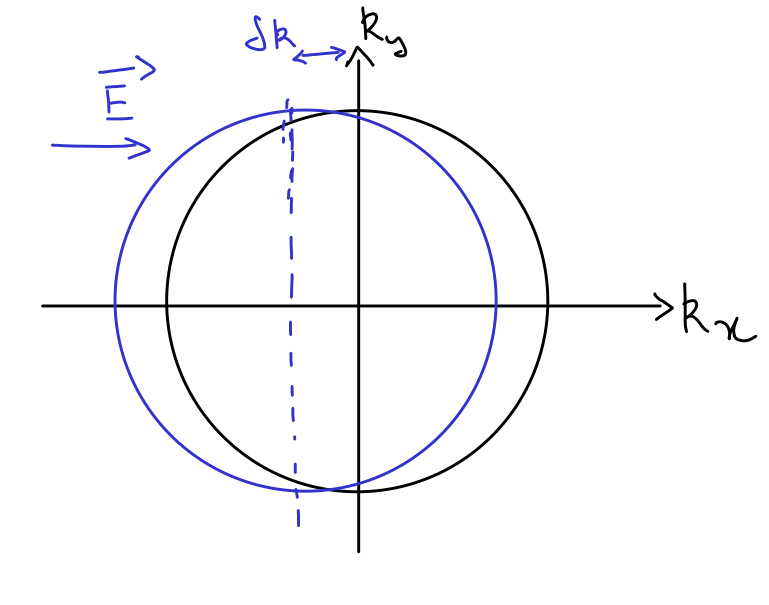
\includegraphics[width=0.8\textwidth]{figures/shift.png}
	\caption{Distribution of free electrons in a uniform electric field}
	\label{fig:figures-shift-png}
\end{figure}

Now that we have some expression for the energy distribution of
charge carriers, we can move on to calculating the current density.
\subsection*{Current Density in the relaxation time approximation}
From equation \ref{current_density}, we have
\begin{equation}
	\begin{split}
		\mathbf{j} &= \int \dd ^3 k \frac{e}{4\pi^3}f\textbf{v}(\textbf{k})\\
			   &= \frac{q}{4\pi^3}\int \dd ^3 k \mathbf{v}_k (f^{0} + \delta f) \\
			   &= \frac{q}{4\pi ^3}\int \dd ^3 k \mathbf{v}_k f^{0} + \frac{q}{4\pi ^3}\int \dd ^3 k \mathbf{v}_k \delta f
	\end{split}
\end{equation}

The first term is just the equilibrium current density, which is zero.
So, we have
\begin{equation}
	\label{current_density_rt}
	\mathbf{j} = 0 + \frac{q}{4\pi ^3}\int d^3k \mathbf{v}_k \delta f
\end{equation}

So, we started from Bloch electrons, applied and electric field
on those electrons. If we plug in $f$ as the FD distro, we should
be able to derive Ohm's law.

Also, even if you didn't have a very nice Fermi sphere, the same
procedure holds for calculating the current density for a more
general Fermi sphere.

We have the FD distro
\begin{equation}
	f^{0} = \frac{1}{1 + \exp((\varepsilon - \mu)\beta)}
\end{equation}
and its derivative
\begin{equation}
	\label{fd_dv}
	\pdv{f^{0}}{\varepsilon} = -\beta f^{0}(1 - f^{0})
\end{equation}
or in the vector form
\begin{equation}
	\label{fd_dvv}
	\grad_k f^{0} = -\beta f^{0}(1 - f^{0})\hcut \mathbf{v}_k
\end{equation}

From (\ref{mult}), we can rewrite (\ref{current_density_rt}) as
\begin{equation}
	\mathbf{j} = \frac{q}{4\pi^3}\int \dd ^3 k \mathbf{v}_k \left( -\frac{q\textbf{E}\tau}{\hcut}\vdot\grad_k f \right).
\end{equation}

Since we are close to equilibrium, as mentioned earlier, we can approximate
$\grad_k f = \grad_k f^{0}$. So, we have
\begin{equation}
	\mathbf{j} = \frac{q}{4\pi^3} \int \dd ^3 k \mathbf{v}_k \left( -\frac{q\textbf{E}\tau}{\hcut}\vdot\grad_kf^{0} \right).
\end{equation}

Substituting  equation (\ref{fd_dvv}) into this, we get
\begin{equation}
	\begin{split}
		\mathbf{j} &= \frac{q}{4\pi^3}\int \dd ^3 k \mathbf{v}_k\left( \frac{q\tau}{\hcut}\beta f^{0}\left( 1 - f^{0} \right) \hcut \mathbf{E}\vdot \mathbf{v}_k \right) \\
			   & = \left[\frac{q^2}{4\pi^3}\int \dd ^3 k \mathbf{v}_k  \otimes \mathbf{v}_k\left( -\pdv{f^{0}}{\varepsilon} \right)\right]\vdot \mathbf{E}
	\end{split}
\end{equation}
where $\otimes$ is the tensor product, i.e.  $A_{ij} = B_iC_j$, collecting
all the indices. Looking at the above equation, we have in the above
equation in the square brackets the conductivity tensory  $\boldsymbol{\sigma}$. 
\begin{equation}
	\label{condtensor}
	\boldsymbol{\sigma} = \frac{q^2}{4\pi^3} \int \dd ^3 k \mathbf{v}_k \otimes \mathbf{v}_k \left( -\pdv{f^{0}}{\varepsilon} \right) 
\end{equation}

We want to recover Drude conductivity. So, we have from equations (\ref{speed}) and (\ref{force}), we have 
\begin{equation}
	\sigma_{ij} = \left[ \frac{q^2}{4\pi^3} \int \dd ^3 k \left( \frac{\hcut}{m} \right) ^2k_i k_j \left( -\pdv{f^{0}}{\varepsilon} \right) \tau  \right]
\end{equation}

The integral is over the entire reciprocal space, so we have
\begin{equation}
	\sigma_{ij} = \begin{cases}
		0\quad \text{if }i\neq j\\
		\left[ \frac{q^2}{4\pi^3}\int \dd k ^3 \left( \frac{\hcut}{m} \right) ^2 k_i^2\left( -\pdv{f^{0}}{\varepsilon} \right)\tau  \right] 
	\end{cases}
\end{equation}

Now, $k^2 = k_i^2 + k_j ^2 + \ldots$. So we can just put $k^2/3$
instead of $k_i ^2$. This gives
\begin{equation}
	\sigma_{ii} = \frac{q^2\tau}{6\pi^3m}\int \dd ^3 k \varepsilon \left( -\pdv{f^{0}}{\varepsilon} \right) 
\end{equation}

We can also write this whole business in terms of the density
of states $g(\varepsilon)$
\[
	\frac{1}{4\pi^3} \int \dd ^3 k = \int g(\varepsilon) \dd \varepsilon
.\] 
\begin{equation}
	\implies \sigma_{ii} = \frac{2q^2}{3m}\int \dd \varepsilon \tau(\varepsilon) \varepsilon
	g(\varepsilon) \left( -\pdv{f^{0}}{\varepsilon} \right) .
\end{equation}

Note that in general $\tau$ is a function of $\varepsilon$.

%%%%% TODO: Homework: Plug in $g(\varepsilon)$ for free electrons in
%%%%% Sommerfeld metal (g(vareps)) = c.sqrt(vareps)

Take a look at figure \ref{fig:figures-fddv-png}. It approaches
a  $\delta$-function as $\beta \to  0$.
\begin{figure}[h]
	\centering
	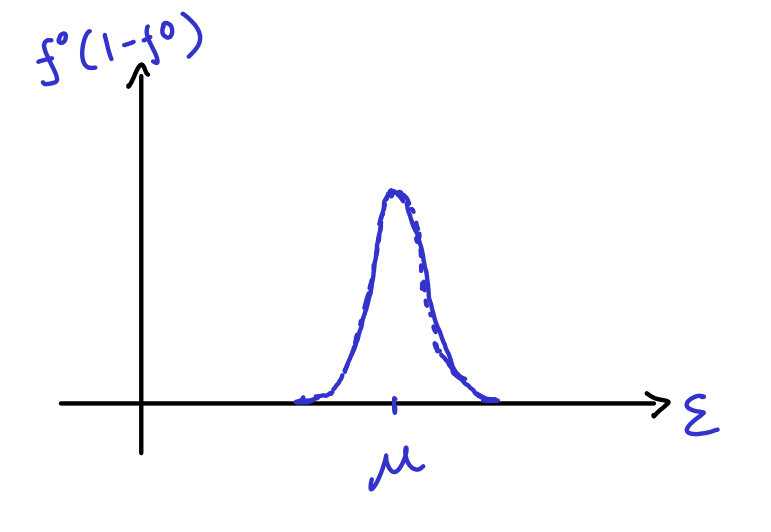
\includegraphics[width=0.8\textwidth]{figures/fddv.png}
	\caption{Derivative of the Fermi-Dirac distribution - FWHM $\sim k_BT$}
	\label{fig:figures-fddv-png}
\end{figure}

%%%%%%%%%% TODO: The Dirac delta thing 
So, we have the Drude conductivity formula 
\begin{equation}
	\begin{pmatrix} j_x\\ j_y\\ j_z \end{pmatrix}
	= \begin{pmatrix} 
	\frac{ne^2\tau}{m} & 0 & 0\\
0 & \frac{ne^2\tau}{m} & 0 \\
0 & 0 & \frac{ne^2\tau}{m}\end{pmatrix} 
\begin{pmatrix} E_x\\E_y\\E_z \end{pmatrix} 
\end{equation}

\subsubsection*{Case 2: $ \mathbf{E} \neq  0, \mathbf{B} \neq  0$ (not necessarily Hall geometry)}
Just one little change
\begin{equation}
	\label{delf}
	\delta f = -\frac{q}{\hcut}\left[ \mathbf{E} + \mathbf{v}_k \times \mathbf{B} \right]\vdot \grad_k  f
\end{equation}

So, now our force term has a $k$-dependence, and hence 
\[
	f \neq  f^{0}(\textbf{k} + \delta \mathbf{k})
,\] 
$\delta k$ itself has a $k$-dependence.

Can we still express $f = f^{0}(\textbf{k} + \delta \mathbf{k}$, where
\begin{equation}
	\label{delk}
	\delta \mathbf{k} = -\frac{\delta \tau}{\hcut}\textbf{z} \vdot\grad_k f^{0}
\end{equation}

where $ \mathbf{z}$ is a vecotr involving $ \mathbf{E} \text{ and } \mathbf{B}$,
but independent of $ \mathbf{k}$ or $ \mathbf{v}_k$.

Consider equation (\ref{delf}), particularly the $ \mathbf{B}$ term
\[
-\frac{q\tau}{\hcut}\left( \mathbf{v}_k \times  \mathbf{B} \right) \vdot\grad_k f
.\] 

Linearize like a good physicist, and check out the first term
\begin{equation}
	\mathbf{v}_k \times  \mathbf{B}\vdot\grad_k f
	= \left( \mathbf{v}_k \times  \mathbf{B} \right) \vdot 
	\left( \grad_k f^{0} + \grad_k \delta f\right) 
\end{equation}

The first term
\begin{equation}
	\label{firstterm}
	\begin{split}
		\left( \mathbf{v}_k \times  \mathbf{B} \right) \vdot \grad_k f^{0} &= \left( \mathbf{v}_k \times  \mathbf{B} \right) \vdot\left( -\left( \pdv{f^{0}}{\varepsilon} \right) \hcut \mathbf{v}_k \right) \\
										 &=	\left( \mathbf{v}_k \times  \mathbf{B} \right) \vdot \left( -\beta f^{0}(1 - f^{0})\hcut \mathbf{v}_k \right) \\
										 &= 0
	\end{split}
\end{equation}

Second term
\begin{equation}
	\label{secondterm}
	\begin{split}
	\grad_k \delta f &=  \grad_k \left( -\frac{q\tau}{\hcut} \mathbf{z}\vdot\grad_k f^{0} \right)\\
	&=  \grad_k \left[ -\frac{q\tau}{\hcut}\textbf{z}\vdot \left( \left( -\pdv{f^{0}}{\varepsilon} \right) \hcut \right) \mathbf{v}_k \right]  \\
	&= -q\tau\grad_k \left[ -\beta f^{0}(1-f^{}) \mathbf{z}\vdot\mathbf{v}_k \right] 
	\end{split}
\end{equation}

	
\end{document}
